% !TEX root = ../main.tex
% File: chapters_part1/chap4_4.tex
% Nội dung cho Chương 4, Phần 4

\section{Các Biến thể Transformer cho Ngữ cảnh dài (Long-Context Transformers)}
\label{sec:long_context_transformers}

\subsection{Vấn đề của Sự chú ý Bậc hai (The Quadratic Bottleneck)}
\label{ssec:quadratic_bottleneck}

Kiến trúc Transformer gốc, với cơ chế Self-Attention đầy đủ (full self-attention), có một hạn chế nghiêm trọng: \textbf{chi phí tính toán và bộ nhớ tăng theo cấp số nhân bậc hai so với độ dài chuỗi ($O(n^2)$)}.

Hãy nhớ lại công thức của Self-Attention: $\text{softmax}\left(\frac{QK^T}{\sqrt{d_k}}\right)V$. Phép nhân ma trận $QK^T$ sẽ tạo ra một \textbf{ma trận chú ý (attention matrix)} có kích thước $n \times n$, trong đó $n$ là độ dài chuỗi.
\begin{itemize}
    \item Nếu $n = 512$, ma trận chú ý có $512^2 \approx 262,000$ phần tử.
    \item Nếu $n = 4096$, ma trận chú ý có $4096^2 \approx 16.7$ triệu phần tử.
    \item Nếu $n = 100,000$ (độ dài một cuốn sách nhỏ), ma trận chú ý sẽ có $10$ tỷ phần tử!
\end{itemize}
Việc lưu trữ và tính toán trên ma trận khổng lồ này là bất khả thi với các phần cứng hiện tại. Đây chính là "nút thắt cổ chai bậc hai", giới hạn hầu hết các mô hình Transformer ban đầu ở độ dài ngữ cảnh là 512 hoặc 1024 token.

Để phá vỡ rào cản này và xử lý các tài liệu dài, các nhà nghiên cứu đã phát triển nhiều phương pháp để làm cho cơ chế chú ý trở nên "hiệu quả" hơn. Hướng tiếp cận phổ biến nhất là \textbf{Chú ý Thưa thớt (Sparse Attention)}.
\subsubsection{Giải pháp từ Kỹ thuật Tối ưu: FlashAttention}
Trước khi đi vào các phương pháp xấp xỉ, cần phải nhắc đến một cuộc cách mạng về mặt triển khai: \textbf{FlashAttention} (Dao et al., 2022)\cite{dao2022flashattention}. FlashAttention không thay đổi kiến trúc Transformer, mà thay đổi \textbf{cách tính toán} cơ chế chú ý trên phần cứng GPU.

\begin{itemize}
    \item \textbf{Vấn đề cốt lõi:} Nút thắt cổ chai của attention không chỉ là số phép tính $O(n^2)$, mà còn là việc truy cập bộ nhớ. Việc đọc và ghi ma trận chú ý $n \times n$ khổng lồ từ bộ nhớ chính (HBM) của GPU ra bộ nhớ đệm (SRAM) cực kỳ chậm.
    \item \textbf{Giải pháp của FlashAttention:} Nó sử dụng các kỹ thuật thông minh như \textbf{tiling} (chia nhỏ ma trận thành các khối) và \textbf{recomputation} (tính toán lại một số giá trị thay vì lưu trữ) để thực hiện toàn bộ phép tính chú ý trong bộ nhớ SRAM tốc độ cao của GPU mà không cần phải ghi toàn bộ ma trận chú ý ra HBM.
    \item \textbf{Kết quả:} FlashAttention có thể tính toán cơ chế chú ý \textbf{chính xác (exact attention)} nhanh hơn tới 3 lần và yêu cầu bộ nhớ chỉ $O(n)$ thay vì $O(n^2)$.
\end{itemize}
Sự ra đời của FlashAttention và các phiên bản kế nhiệm (FlashAttention-2) đã giúp các mô hình Transformer gốc có thể xử lý ngữ cảnh dài hơn đáng kể (ví dụ, từ 2k lên 8k, 16k, hoặc 32k) mà không cần phải thay đổi kiến trúc. Nó là một trong những nền tảng kỹ thuật quan trọng nhất cho các LLM hiện đại.
\subsection{Lý thuyết về Chú ý Thưa thớt (Sparse Attention)}
\label{ssec:sparse_attention_theory}

\subsubsection{Trực giác cốt lõi}
Ý tưởng trung tâm của Sparse Attention là: \textbf{một token không cần phải chú ý đến tất cả các token khác trong chuỗi}. Hầu hết thông tin quan trọng đều đến từ các token lân cận (ngữ cảnh cục bộ) hoặc một vài token "quan trọng" đặc biệt trên toàn chuỗi.

Thay vì tính toán một ma trận chú ý $n \times n$ dày đặc, các mô hình Sparse Attention chỉ tính toán và lưu trữ một số lượng nhỏ các điểm chú ý, làm cho chi phí giảm từ $O(n^2)$ xuống gần như tuyến tính, $O(n \log n)$ hoặc $O(n)$.

\begin{center}
    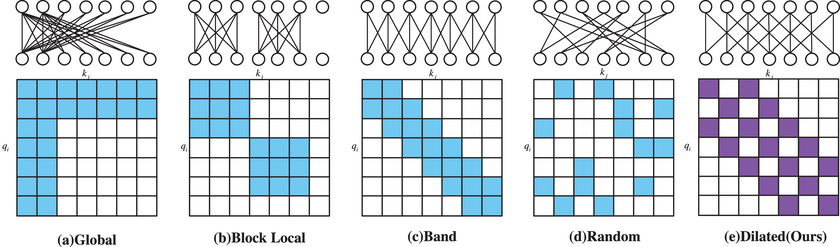
\includegraphics[width=1.0\textwidth]{sparse_attention_patterns.png}
    \captionof{figure}{So sánh các mẫu chú ý thưa (sparse attention). 
    (a) Chú ý toàn cục (Global). 
    (b) Chú ý theo khối cục bộ (Block Local). 
    (c) Chú ý theo dải (Band), hay còn gọi là cửa sổ trượt (Sliding Window). 
    (d) Chú ý ngẫu nhiên (Random). 
    (e) Chú ý giãn cách (Dilated). 
    Các mô hình như Longformer và BigBird thường kết hợp các mẫu này.}
    \label{fig:sparse_attention_patterns}
\end{center}

Hai mô hình tiên phong và tiêu biểu nhất cho trường phái này là Longformer và BigBird.

\subsubsection{Longformer: Kết hợp Cửa sổ trượt và Chú ý Toàn cục}
Longformer (Beltagy et al., 2020) \cite{beltagy2020longformer} đề xuất một mẫu chú ý kết hợp ba thành phần:

\paragraph{1. Chú ý Cửa sổ trượt (Sliding Window Attention)}
\begin{itemize}
    \item \textbf{Cơ chế:} Mỗi token chỉ chú ý đến một cửa sổ có kích thước cố định $w$ gồm các token xung quanh nó (ví dụ: $w/2$ token bên trái và $w/2$ token bên phải).
    \item \textbf{Mục đích:} Nắm bắt ngữ cảnh cục bộ, tương tự như trong các mô hình CNN. Đây là phần lớn các kết nối chú ý trong mô hình.
\end{itemize}

\paragraph{2. Chú ý Cửa sổ trượt Giãn cách (Dilated Sliding Window)}
\begin{itemize}
    \item \textbf{Cơ chế:} Để mở rộng "trường tiếp nhận" (receptive field) mà không tăng chi phí, Longformer sử dụng các cửa sổ trượt có "lỗ" (gaps) ở các lớp khác nhau. Ví dụ, ở một lớp, cửa sổ có thể chú ý đến các token cách nhau 1 vị trí, ở lớp khác, cách nhau 2 vị trí, v.v.
    \item \textbf{Mục đích:} Giúp thông tin từ các token xa hơn có thể được tích hợp vào biểu diễn của một token mà không cần kết nối trực tiếp.
\end{itemize}

\paragraph{3. Chú ý Toàn cục (Global Attention)}
\begin{itemize}
    \item \textbf{Cơ chế:} Một số ít các token được chọn trước được phép chú ý đến \textbf{tất cả} các token khác trong chuỗi, và ngược lại, tất cả các token khác cũng được phép chú ý đến chúng.
    \item \textbf{Mục đích:} Các token toàn cục này hoạt động như một "trung tâm thông tin", tổng hợp và phân phối thông tin trên toàn bộ chuỗi. Các token này thường được chọn một cách đặc biệt, ví dụ như token `[CLS]` trong các tác vụ phân loại.
\end{itemize}

Bằng cách kết hợp các mẫu này, Longformer giảm độ phức tạp tính toán xuống $O(n \cdot w)$, gần như tuyến tính với độ dài chuỗi $n$, cho phép nó xử lý các chuỗi lên tới 4096 token hoặc hơn.

\subsubsection{BigBird: Thêm các Mẫu Chú ý Ngẫu nhiên}
BigBird (Zaheer et al., 2020) \cite{zaheer2020big} có triết lý tương tự Longformer nhưng bổ sung thêm một thành phần:
\begin{itemize}
    \item Nó cũng sử dụng \textbf{Chú ý Cửa sổ trượt} và \textbf{Chú ý Toàn cục}.
    \item Điểm mới lạ là nó thêm vào \textbf{Chú ý Ngẫu nhiên (Random Attention)}. Mỗi token sẽ chú ý đến một số lượng nhỏ $r$ các token được chọn ngẫu nhiên từ toàn bộ chuỗi.
\end{itemize}
Các tác giả đã chứng minh về mặt lý thuyết rằng một mô hình kết hợp ba loại chú ý này (cửa sổ, toàn cục, ngẫu nhiên) có thể xấp xỉ được các thuộc tính của cơ chế chú ý đầy đủ và là một bộ xấp xỉ hàm phổ quát (universal function approximator).

\subsection{Các phương pháp khác: Thoát khỏi Self-Attention Bậc hai}
\label{ssec:other_long_context_methods}

Sparse Attention là một hướng tiếp cận, nhưng không phải là duy nhất. Một hướng đi khác, cấp tiến hơn, là đặt câu hỏi: "Liệu chúng ta có thực sự cần cơ chế chú ý bậc hai không?". Điều này đã dẫn đến sự ra đời của các kiến trúc hoàn toàn mới.
\subsubsection{Cải tiến Mã hóa Vị trí (Positional Encoding)}
Một hướng quan trọng khác để giúp Transformer xử lý ngữ cảnh dài là cải tiến cách nó hiểu về vị trí của token.
\paragraph{ALiBi (Attention with Linear Biases)}
Thay vì thêm mã hóa vị trí vào embedding, ALiBi \cite{press2021train} trực tiếp sửa đổi ma trận điểm chú ý.
\begin{itemize}
    \item \textbf{Cơ chế:} Trước khi qua softmax, điểm chú ý giữa token $i$ và $j$ sẽ bị trừ đi một "án phạt" (penalty) tỷ lệ thuận với khoảng cách của chúng: $\text{score}(i, j) - m \cdot |i - j|$. Trong đó, $m$ là một hệ số học được cho mỗi "đầu" chú ý.
    \item \textbf{Trực giác:} "Các từ càng xa nhau thì càng ít liên quan".
    \item \textbf{Lợi ích:} ALiBi cho thấy khả năng \textbf{ngoại suy (extrapolation)} ấn tượng. Một mô hình được huấn luyện trên ngữ cảnh 2048 token với ALiBi có thể hoạt động tốt trên ngữ cảnh 4096 token hoặc dài hơn mà không cần fine-tuning.
\end{itemize}

\paragraph{RoPE Scaling}
Các mô hình sử dụng Rotary Position Embedding (RoPE) như Llama thường gặp khó khăn khi ngoại suy ra các chuỗi dài hơn độ dài huấn luyện. Các kỹ thuật RoPE Scaling giải quyết vấn đề này.
\begin{itemize}
    \item \textbf{Vấn đề:} RoPE sử dụng các hàm sin/cos với tần số phụ thuộc vào vị trí. Khi vị trí vượt quá giới hạn huấn luyện, các tần số này bắt đầu lặp lại hoặc tạo ra các mẫu không ổn định.
    \item \textbf{Giải pháp (ví dụ:\cite{bloc972023ntkaware}, YaRN \cite{peng2023yarn}):} Các kỹ thuật này sửa đổi "bước sóng" (wavelength) của các hàm sin/cos, về cơ bản là "kéo dãn" không gian vị trí để có thể chứa các chuỗi dài hơn mà không phá vỡ các mối quan hệ tương đối đã học được ở cự ly gần.
\end{itemize}
\subsubsection{Mô hình Trạng thái (State Space Models - SSMs) và Mamba}
Đây là một trong những hướng nghiên cứu thú vị và hứa hẹn nhất gần đây.

\paragraph{Nguồn gốc từ Lý thuyết Điều khiển}
SSMs có nguồn gốc từ lý thuyết điều khiển và xử lý tín hiệu. Chúng được thiết kế để mô hình hóa các hệ thống động liên tục. Ý tưởng cốt lõi là duy trì một \textbf{trạng thái ẩn (state) $h(t)$ nhỏ, có kích thước cố định}, và cập nhật nó một cách liên tục theo thời gian dựa trên đầu vào $x(t)$.
$$ h'(t) = \mathbf{A}h(t) + \mathbf{B}x(t) $$
$$ y(t) = \mathbf{C}h(t) + \mathbf{D}x(t) $$
Trong đó $\mathbf{A, B, C, D}$ là các ma trận tham số.

\paragraph{Thách thức và Giải pháp}
Việc áp dụng trực tiếp SSMs vào học sâu là rất khó khăn về mặt tính toán. Các mô hình như S4 (Structured State Space for Sequence Modeling) \cite{gu2021efficiently} đã giải quyết vấn đề này bằng cách tìm ra một cách hiệu quả để "rời rạc hóa" (discretize) các công thức liên tục này, cho phép chúng được tính toán như một phép tích chập lớn trong quá trình huấn luyện (rất nhanh và song song) và như một RNN trong quá trình suy luận (hiệu quả về bộ nhớ).

\paragraph{Mamba: SSMs có Chọn lọc (Selective SSMs)}
Mamba (Gu \& Dao, 2023) \cite{gu2023mamba} là một bước đột phá lớn dựa trên SSMs. Nó nhận ra rằng một hạn chế của các SSMs trước đó là các ma trận $\mathbf{A, B, C, D}$ là \textbf{cố định}, không phụ thuộc vào đầu vào. Điều này có nghĩa là mô hình không thể thay đổi hành vi của mình dựa trên nội dung cụ thể mà nó đang xử lý.

Mamba đã giải quyết vấn đề này bằng cách làm cho các ma trận $\mathbf{B, C}$ và một tham số bước $\Delta$ \textbf{phụ thuộc vào đầu vào (input-dependent)}.
\paragraph{So sánh SSMs và RNNs truyền thống}
Ở chế độ suy luận, SSM hoạt động tuần tự giống như một RNN. Tuy nhiên, có một sự khác biệt cốt lõi:
\begin{itemize}
    \item \textbf{RNNs (LSTM/GRU):} Việc cập nhật trạng thái ẩn đi qua các cổng phi tuyến phức tạp (sigmoid, tanh). Các cổng này, mặc dù mạnh mẽ, lại làm cho gradient khó chảy ngược qua các chuỗi dài và khó song song hóa trong quá trình huấn luyện.
    \item \textbf{SSMs:} Việc cập nhật trạng thái về bản chất là \textbf{tuyến tính} ($h'(t) = \mathbf{A}h(t) + \dots$). Bản chất tuyến tính này, kết hợp với các ma trận được cấu trúc đặc biệt, cho phép gradient chảy ngược qua các chuỗi rất dài mà không bị triệt tiêu, đồng thời cho phép nó được biến đổi thành một phép tích chập song song hóa được khi huấn luyện.
\end{itemize}
Mamba kế thừa những ưu điểm này và thêm vào đó khả năng chọn lọc thông tin, tạo ra một kiến trúc vừa hiệu quả vừa mạnh mẽ.
\begin{tcolorbox}[
    title=Cơ chế Chọn lọc của Mamba,
    colback=green!5!white, colframe=green!60!black, fonttitle=\bfseries
]
Mamba có khả năng \textbf{chọn lọc} thông tin. Dựa trên token đầu vào hiện tại, nó có thể quyết định:
\begin{enumerate}
    \item \textbf{Tập trung:} Nếu một thông tin quan trọng xuất hiện, nó có thể "mở cổng" để cho thông tin đó đi vào trạng thái ẩn.
    \item \textbf{Lãng quên:} Nếu thông tin hiện tại không còn liên quan, nó có thể "nén" hoặc "quên" đi trạng thái ẩn cũ và đặt lại.
\end{enumerate}
Khả năng chọn lọc này cho phép Mamba nén ngữ cảnh một cách linh hoạt, chỉ giữ lại những gì cần thiết, một khả năng mà các mô hình tích chập hay RNN tuyến tính trước đó không có được.
\end{tcolorbox}

\paragraph{Ưu điểm của Mamba so với Transformer}
\begin{itemize}
    \item \textbf{Độ phức tạp tuyến tính:} Cả huấn luyện và suy luận đều có độ phức tạp $O(n)$, nhanh hơn nhiều so với $O(n^2)$ của Transformer.
    \item \textbf{Suy luận nhanh:} Tốc độ suy luận (sinh từ mới) nhanh hơn Transformer vì nó không cần tính toán lại ma trận chú ý khổng lồ ở mỗi bước.
\end{itemize}
Mamba và các kiến trúc dựa trên SSMs đang nổi lên như một đối thủ cạnh tranh thực sự với Transformer, đặc biệt là trong các kịch bản yêu cầu ngữ cảnh cực dài và hiệu quả tính toán cao.

\subsubsection{Các hướng tiếp cận khác}
Ngoài ra, còn có các hướng tiếp cận khác như:
\begin{itemize}
    \item \textbf{Tích chập có cửa sổ lớn (Large Kernel Convolutions):} Sử dụng các lớp tích chập 1D nhưng với kích thước kernel rất lớn để mô phỏng sự tương tác tầm xa.
    \item \textbf{Phương pháp đệ quy (Recurrence):} Cố gắng đưa trở lại một số dạng của cơ chế RNN để nén thông tin từ các đoạn (chunks) văn bản dài.
\end{itemize}

Việc xử lý ngữ cảnh dài vẫn là một trong những lĩnh vực nghiên cứu năng động nhất, hứa hẹn sẽ mở khóa nhiều khả năng mới cho các mô hình ngôn ngữ trong tương lai.